\Gls{ibc} systems are feedback control systems that rely on image-based sensing data obtained from (a) camera sensor(s). Advancements in camera technologies, image-processing algorithms and parallel computing heterogeneous platforms have made \gls{ibc} systems immensely popular in automotive applications~\cite{bengler2014three} like \glspl{adas}, autonomous driving systems, etc. 
However, the enormous compute requirements of \gls{ibc} systems make them challenging to be implemented on such platforms without sacrificing control performance. The focus of this work is to improve the compute and memory efficiency of \gls{ibc} systems (implemented on embedded platforms) by introducing approximations, without sacrificing the control performance. In essence, approximation reduces the compute workload at the cost of additional sensor noise. However, the inherent error resilience of \gls{ibc} systems allows the introduction of this additional sensor noise without sacrificing control performance.
\par A typical \gls{ibc} system consists of a sensing task (\taskS), a control task (\taskC) and an actuation task (\taskA) (see Fig. \ref{fig:lkas_tasks}). \taskS\ involves pre-processing the image frames obtained from the camera sensor and extracting application-specific features. \taskC\ applies the control algorithm using these extracted features and \taskA\ implements the control decisions in the environment. A \gls{wcet} analysis shows that the execution time of \taskS\ is orders of magnitude higher than those of \taskC\ and \taskA, thus, resulting in a long sensing-to-actuation delay $\tau$ (see Fig.\ \ref{fig:lkas_tasks}). 

% \vspace{-10pt}
\begin{figure}[ht]
	\centering
	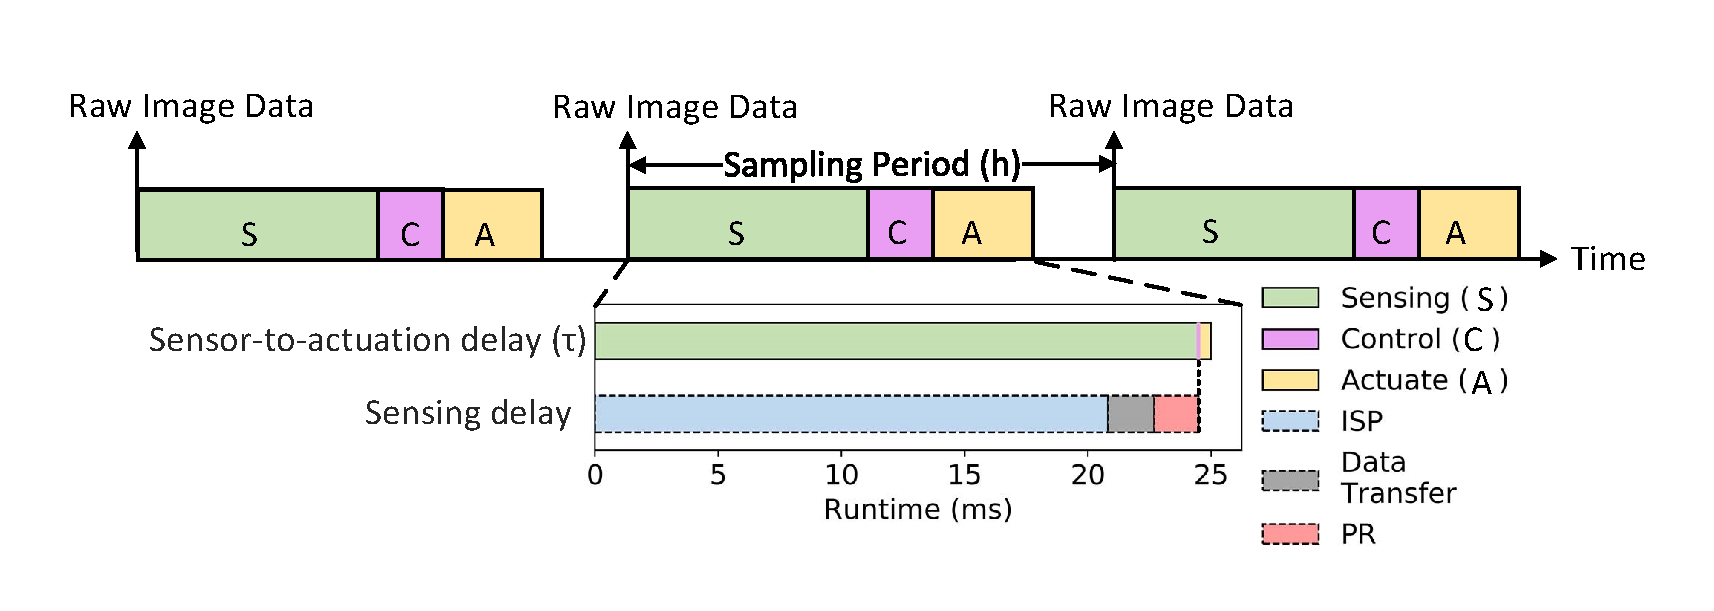
\includegraphics[width= \textwidth]{figs/profiling_lkas1_v3.pdf}
	\caption{{Tasks in an \gls{ibc} system: Runtimes for the sub-tasks are shown for a \gls{lkas} implemented on NVIDIA AGX Xavier embedded platform \cite{nvidiaAGX} (8-core \gls{cpu}+\gls{gpu}). Runtimes are shown for 512 $\times$ 256 resolution images.}}
	\label{fig:lkas_tasks}
% 	\vspace{-10pt}
\end{figure}

\par The \gls{qoc} of an \gls{ibc} system depends on the sensing-to-actuation delay $\tau$. Smaller $\tau$ results in a lower sampling period for the controller, which improves the overall \gls{qoc}. The sensing task (\taskS) is the main bottleneck in lowering $\tau$.
Besides through parallelisation, as already explained in Chapter~\ref{chap:parallelisation}, approximate computing can reduce the \gls{wcet} of \taskS\ by reducing the compute  while introducing sensor noise. \gls{ibc} systems are equipped with \gls{isp} pipelines optimized for human visual consumption; control algorithms, which are inherently resilient to sensor noise, do not need the high-quality images produced by these pipelines. \textit{The work in this chapter focuses on system approximation by reducing the compute workload of the \gls{isp} and the data transfer traffic to off-chip memory, resulting in better \gls{qoc} of the overall system.}

\par  Reduced compute workloads due to approximations introduce new task mapping opportunities for parallelised sensing tasks. Approximate tasks can be mapped to slower power-efficient platform cores, while operating the controller at the same sampling period, guaranteeing proper system functionality.   
The combined impact of both approximations and platform mappings was not explored in the literature prior to this work. 
\textit{The work in this chapter explores the interplay between the degree of approximation and different platform mappings while analyzing their impact on \gls{qoc} and memory efficiency of the entire \gls{ibc} system}. 

A point to consider is that approximation introduces errors in the measurement of states of the system.
\textit{We propose a method to design an approximation-aware optimal \gls{lqg} controller by modelling the approximation error as sensor noise}. 

\par \gls{ibc} systems operate under different environmental scenarios \cite{env_cond}. For example, image feedback at night requires a different nature of processing compared to the same during the day in \gls{adas}. These scenarios significantly influence the degree of approximation that can be tolerated without destabilizing the system. The robustness study on how approximations impact the \gls{ibc} performance under different environmental scenarios is essential but is was also not addressed in prior literature. 
\textit{For different environmental conditions, we design different approximation-aware controllers and show that our approach is robust to different environmental scenarios by performing a \gls{fp} analysis for the approximate system using Monte-Carlo simulations.}   

In summary, our approach takes into account various artefacts of approximation-in-the-loop in terms of platform mapping and controller design, while considering robustness to failures. We refer to this approach as approximation-aware \gls{ibc} design. 
The key contributions of this work are as follows:

\begin{enumerate}
    \item \textit{\Gls{imacs} framework: }
    The \gls{imacs} framework\footnote{The \gls{imacs} framework is open sourced and can be accessed on github: https://github.com/sajid-mohamed/imacs} (Section \ref{lkas_hil}) helps to test and evaluate the impact of approximation in closed-loop feedback systems.
    First, the resilience of the given \gls{ibc} system to different approximation choices is analysed. Second, for each approximation choice, the sensing delay is computed, and the error due to approximations is quantified using the \gls{imacs} framework.
    
    \item \textit{Optimized approximation-aware \gls{ibc}\footnote{Our approximation-aware design framework is open sourced and can be accessed on github: https://github.com/sayandipde/approx\_ibc}: } 
    We illustrate the potential of exploiting the inherent error resilience of \gls{ibc} systems by performing coarse-grained computation skipping in the \gls{isp} (compute-centric approximation, Section \ref{ss_optim_1}). Further, we introduce two optimizations on top. First, we perform a data-centric approximation by varying the degree of lossy compression post-\gls{isp} (Section~\ref{ss_optim2}), which  shows a memory reduction of up to 88\%, and hence a performance improvement. Second, we design an approximation-aware \gls{lqg} controller that models the errors due to approximation as sensor noise (Section~\ref{lqg_control}). These approximations and optimizations turn out to substantially improve the overall \gls{qoc} compared to the accurate implementation. 
    
   \item \textit{Scenario-awareness: }
    Environmental scenarios significantly influence the degree of approximation that can be tolerated without destabilizing an \gls{ibc} system. We perform scenario-specific optimization considering six different environmental scenarios relevant for \gls{lkas}, i.e., \textit{day, night, dawn, dusk, fog, snow}. We show that scenario-specific approximation decisions improve the overall \gls{qoc} (Section~\ref{robust}).
    
    \item \textit{Failure probability analysis: }Applicability of our proposed approach to safety-critical systems (such as \gls{lkas}) require \gls{fp} analysis to comply with well-accepted safety margins \cite{fault_tree}. 
    In this work, we perform \gls{fp} analysis based on Monte-Carlo simulations to show the robustness of approximate \gls{ibc} systems designed using our approach (Section \ref{failure}).
    
\end{enumerate}

Improving the runtime performance of the sensing task through approximations is complementary to the \gls{spade} approach presented in earlier chapters. 
The \gls{spade} approach for an industrial platform (explained in Section \ref{sec:ch7_SPADeIndustrial}) already uses the approximated sensing algorithm introduced in this chapter. The approximation-aware design offers alternatives in terms of sensing (with approximate \gls{isp}) and controller (i.e., approximation-aware controller) in the \gls{spade} flow.